\documentclass[onecolumn]{article}

%Titling
    \usepackage[compact]{titlesec}
    \titlespacing{\section}{0pt}{3ex}{2ex}
    \titlespacing{\subsection}{0pt}{2ex}{1ex}
    \titlespacing{\subsubsection}{0pt}{1ex}{0.5ex}
\titleformat*{\section}{\Large\scshape}
\titleformat*{\subsection}{\Large}
\titleformat{\subsubsection}
  {\normalfont\bfseries}{\thesubsection}{1em}{}
  
%Page size
	\addtolength{\oddsidemargin}{-.875in}
	\addtolength{\evensidemargin}{-.875in}
	\addtolength{\textwidth}{1.75in}

	\addtolength{\topmargin}{-.875in}
	\addtolength{\textheight}{1.75in}
	
	\parskip=.1cm

\usepackage{graphicx}
\graphicspath{ {figures/} }
\usepackage[T1]{fontenc}
\usepackage{lmodern}
\usepackage{float}
\usepackage[table]{xcolor}
\usepackage{multirow}
\usepackage{tabularx} 
\usepackage[table]{xcolor}
\usepackage[font=small,labelfont=bf]{caption}
\usepackage{textcomp}
\usepackage{gensymb}
\usepackage{lineno}
\usepackage{amsmath}
\usepackage{blindtext}
\usepackage{texshade}
\usepackage{bigdelim}
\usepackage{textgreek}
\usepackage{multicol}

% tikz setup
\usepackage{tikz}
\usetikzlibrary{shapes,arrows}
\newcommand*{\h}{\hspace{5pt}}% for indentation
\newcommand*{\hh}{\h\h}% double indentation


%Citations
\usepackage[authoryear]{natbib}
\setcitestyle{authoryear,open={(},close={)}}
\renewcommand{\bibname}{References}

\usepackage[allbordercolors = white, linkcolor = blue, citecolor = blue, colorlinks = true]{hyperref}
\usepackage[nameinlink]{cleveref}

%titling
\title{Modelling Uncertainty in the Risk of Intensive Care Unit Readmission I: Data Extraction and Modelling}
\date{\today}
\author{Ben Cooper}


\begin{document}
\maketitle

\section{Introduction}

% Brief background on ICU risk stuff
Unplanned readmission to an intensive care unit (ICU) during the same hospital admission is a relatively common event, affecting between 1.3\% and 13.7\% of all ICU patients \citep{Elliott2014}. Not only do readmissions to ICU represent a substantial strain on hospital resources, but also readmitted patients tend to have worse prognoses, increased length of ICU stay, and greater risks of morbidity and mortality \citep{MarkaziMoghaddam2020}. Despite this, the precise factors contributing to ICU readmission risk remain unclear. Several models for risk prediction have been developed which tend to use very different variable sets, and no model has been widely externally validated. Accordingly, this project does not aim to develop or validate a novel model for ICU readmission, but to tackle an issue that affects the implementation and interpretation of all risk prediction models - how to deal with missing or incomplete data in the predictor variables \citep{Steyerberg2008}.

\subsection{Scope and Aims of Phase I}

This document provides a written overview of the first phase of the project. The aims of this phase were twofold:

\begin{enumerate}
\item To extract a dataset from the MIMIC-III database of surgical ICU patients, consisting of a clearly defined outcome measure (ICU readmission), and a range of predictors.
\item To compare the performance of a range of published models for the prediction of ICU readmission risk and identify the best model to take forward. This will form the prediction model at the core of a system for quantifying uncertainty and dealing with missing data.
\end{enumerate}


\subsection{Readmission prediction models}

% Overview of structure, strengths and shortcomings of each model
This report will investigate five models for ICU risk prediction. I will give a brief overview of all five here. Further details on their predictors, statistical approaches and validations are given in \Cref{CandidateModels}.
% APACHE-II
The first `model' is the APACHE-II scoring system devised by \cite{Knaus1985}. `Model' is used in inverted commas, as this model was not designed for predicting ICU readmission risk, but instead is a general system to score the severity of a patient's condition using 12 routine physiological variables, age, and medical history. Increasing APACHE-II score has been shown to correlate well with increasing risk of in-hospital mortality for ICU patients. 
% Frost
\cite{Frost2010} used a logistic regression model to develop a nomogram for predicting ICU readmission risk based on 14,952 patients in a single hospital in Australia. Unfortunately, as they do not present the coefficients from their model directly, only in the form of the nomogram, several of these coefficients can only be approximated, which may hinder external validation of the model.

% Fialho
\cite{Fialho2012} developed a model using data mining and fuzzy logic approaches with the MIMIC-II database, precursor to the MIMIC-III used here. Their model focusses on the values of physiological variables during the 24 h before discharge. The fuzzy rules provide a significant barrier to external validation, however.
% Martin
\cite{Martin2018} also developed their model into a nomogram, but unlike Frost, also provided coefficients and a precise formula to generate risk estimates. Their model used 3,109 patients in a single academic centre, and narrowed an initial 179 candidate variables down to 7 variables, covering demographics, physiological measurements and medical history.
% Hammer focussed on modifiable variables
Finally, \cite{Hammer2020} developed the `RISC' score (Readmission to the
Intensive care unit in Surgical Critical care patients, henceforth simply called `Hammer' for consistency with other models) using logistic regression. Their model aimed to include a number of modifiable variables to aid its use as a clinical tool.

\section{Methods}

\subsection{Data Source}

% Overview of MIMIC data
This work uses the open-access MIMIC-III critical care database \citep{Johnson2016}, which comprises ICU stay information for 61,532 adult patients at the Beth Israel Deaconess Medical Centre between June 2001 and October 2012. The database includes information such as demographics, vital sign measurements made at the bedside ($\sim$1 data point per hour), laboratory test results, procedures, medications, caregiver notes, imaging reports, and mortality (both in and out of hospital).

\subsection{Inclusion criteria}

% Workflow in extract_patients & preprocess_data
An overview of inclusion and exclusion criteria is shown in \Cref{Flowchart}. In brief, we initially include all patients admitted under or transferred to a surgical service, and who underwent a surgical procedure either during or prior to an ICU stay. We exclude patients with invalid surgical procedure codes, or procedure types with <20 patients in the dataset. We also exclude patients whose surgical procedure took place after their last ICU stay, or who died during the same hospital admission as their ICU stay. Finally, we exclude patients with data in any of the following categories:

\begin{itemize}
\item Missing entire hospital record
\item Missing assessment data for predictors
\item Missing measurement data for predictors within 24 h prior to ICU discharge
\item Physiologically impossible or implausible measurements
\end{itemize}

% Flowchart------------
\begin{figure}
\centering
\label{Flowchart}
  \caption{Flowchart of inclusion and exclusion criteria for patients in the dataset, alongside sample sizes at each step.}
  % setting the typeface to sans serif and the font size to small
  % the scope local to the environment
  \sffamily
  \footnotesize
  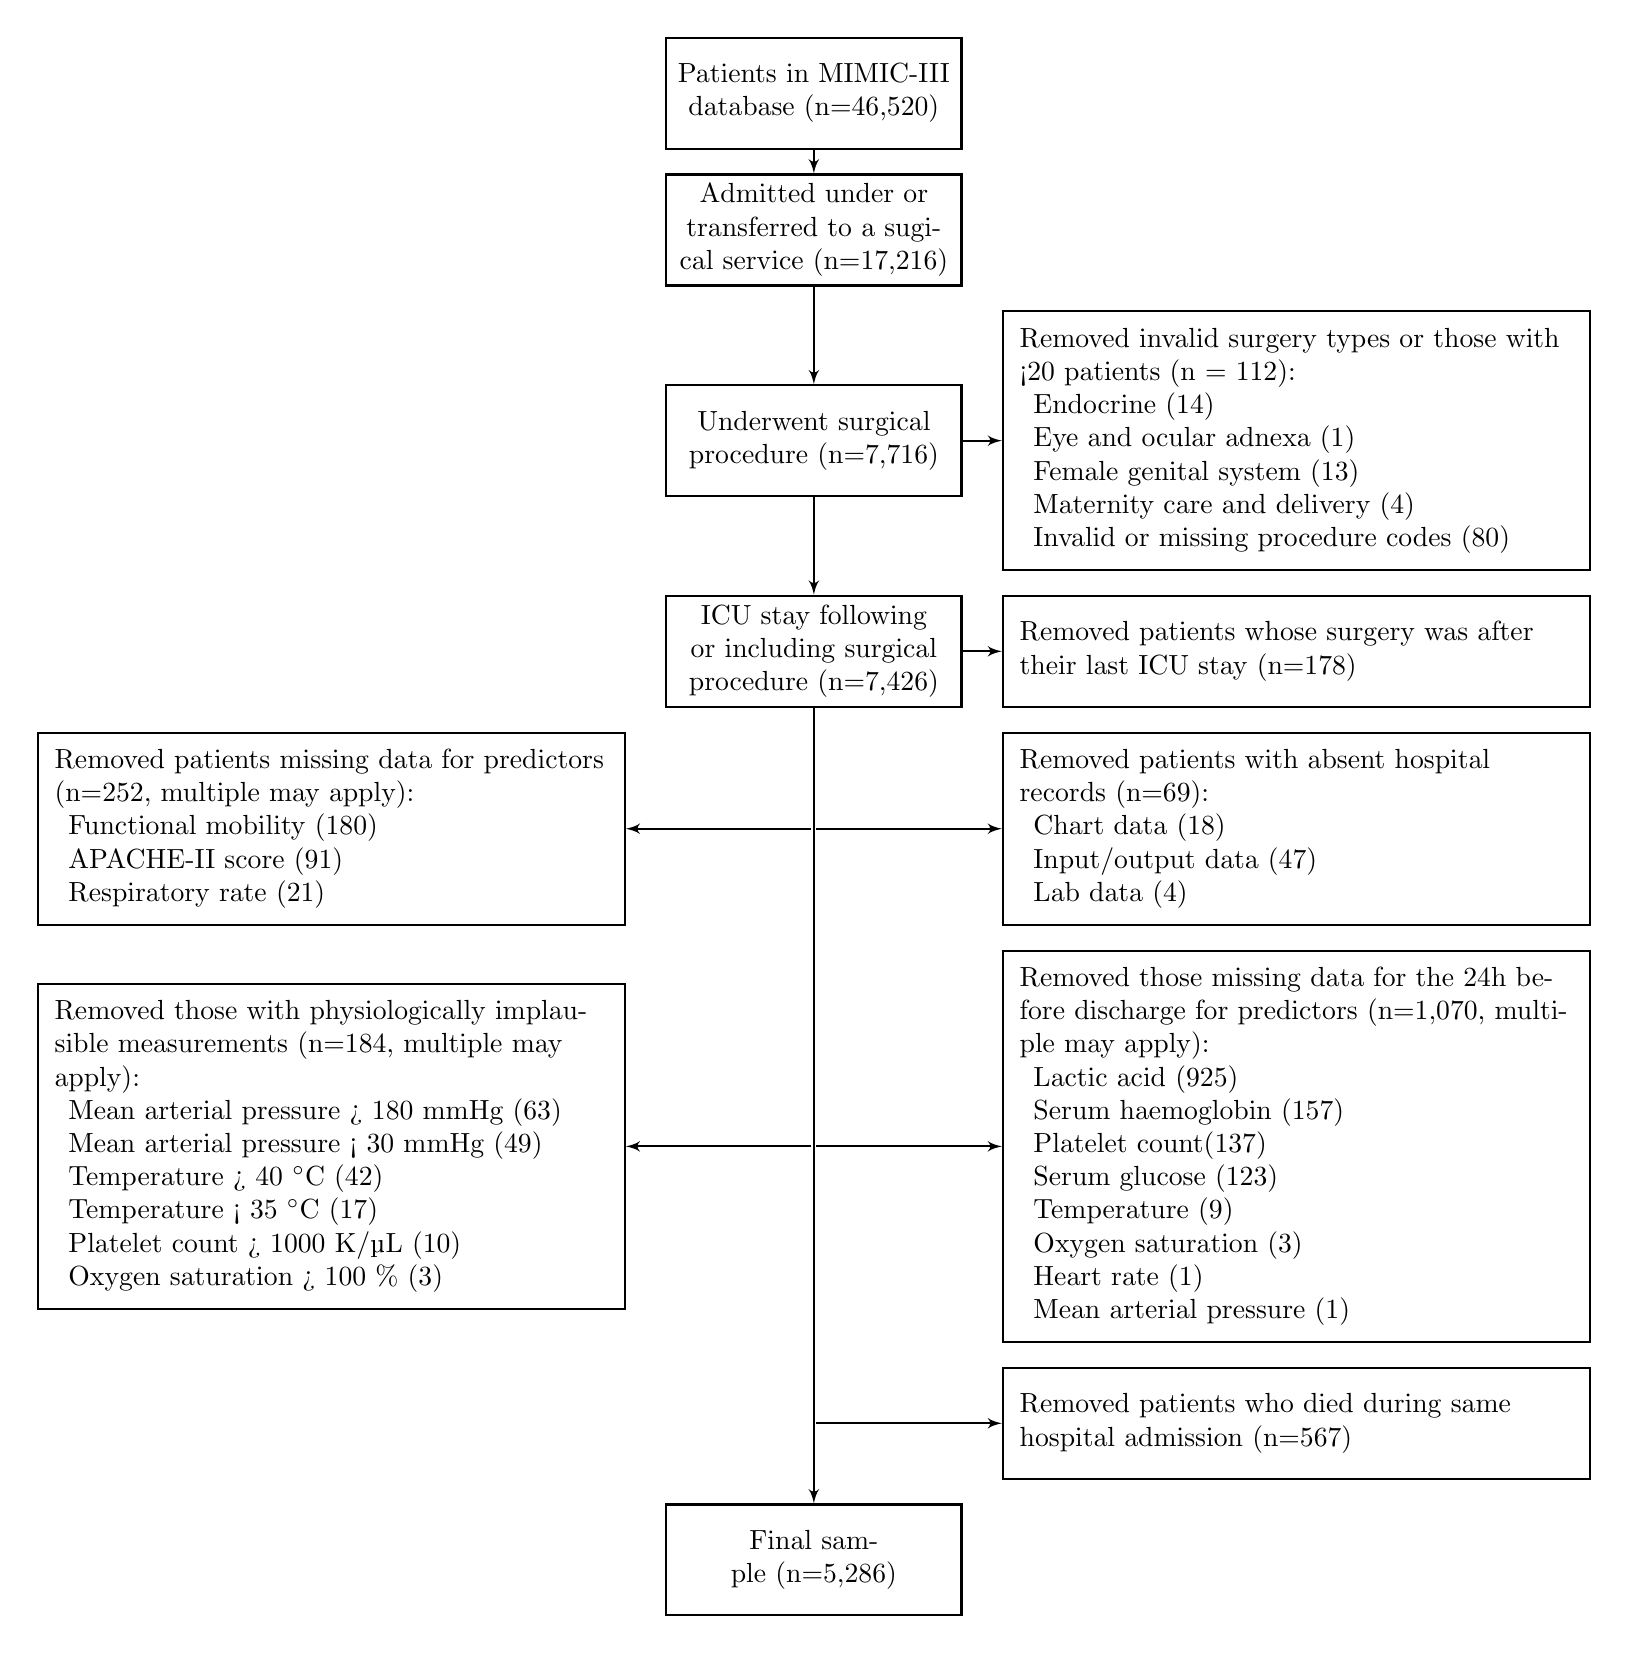
\begin{tikzpicture}[auto,
    block_center/.style ={rectangle, draw=black, thick, fill=white,
      text width=10em, text centered,
      minimum height=4em},
    block_left/.style ={rectangle, draw=black, thick, fill=white,
      text width=20em, text ragged, minimum height=4em, inner sep=6pt},
      line/.style ={draw, thick, -latex', shorten >=0pt},
          block_noborder/.style ={rectangle, draw=none, thick, fill=none,
      text width=-4em, text centered, minimum height=1em}]
    % outlining the flowchart using the PGF/TikZ matrix funtion
    \matrix [column sep=5mm,row sep=3mm] {
      % row 1
      & \node [block_center] (full) {Patients in MIMIC-III database (n=46,520)};\\
      % row 2
      &\node [block_center] (service) {Admitted under or transferred to a sugical service (n=17,216)}; \\
      % row 3
      &\node [block_center] (procedure) {Underwent surgical procedure (n=7,716)};       
      & \node [block_left] (invalidprocedure) {Removed invalid surgery types or those with <20 patients (n = 112): \\
        \h Endocrine (14)\\
        \h Eye and ocular adnexa (1)\\
        \h Female genital system (13)\\
        \h Maternity care and delivery (4)\\
        \h Invalid or missing procedure codes (80)
        }; \\
      % row 4
        &\node [block_center] (icuprocedure) {ICU stay following or including surgical procedure (n=7,426)};       
      & \node [block_left] (procedure_after_icu) {Removed patients whose surgery was after their last ICU stay (n=178)}; \\
      % row 5  
        \node [block_left] (missing_predictors) {Removed patients missing data for predictors (n=252, multiple may apply):\\
		\h Functional mobility (180)\\
		\h APACHE-II score (91)\\
		 \h Respiratory rate (21)}; &
       \node [block_noborder] (hidden_r5) {};&
      \node [block_left] (absent_charts) {Removed patients with absent hospital records (n=69): \\
        \h Chart data (18)\\
        \h Input/output data (47)\\
        \h Lab data (4)
        }; \\  
        % row 6 
        \node [block_left] (implausible) {Removed those with physiologically implausible measurements (n=184, multiple may apply): \\
		\h Mean arterial pressure > 180 mmHg (63)\\
	 	\h Mean arterial pressure < 30 mmHg (49)\\
		\h Temperature > 40 $^\circ$C (42)\\
		\h Temperature < 35 $^\circ$C (17)\\
		\h Platelet count > 1000 K/$\micro$L (10)\\
		\h Oxygen saturation > 100 \% (3)
        };   &
           \node [block_noborder] (hidden_r6) {};&
      \node [block_left] (missing_24h) {Removed those missing data for the 24h before discharge for predictors (n=1,070, multiple may apply): \\
		\h Lactic acid (925)\\
		\h Serum haemoglobin (157)\\
		\h Platelet count(137)\\
		\h Serum glucose (123)\\
		\h Temperature (9)\\
		\h Oxygen saturation (3)\\
		\h Heart rate (1)\\
		\h Mean arterial pressure (1)
        }; \\  
        % row 7  
       &
       \node [block_noborder] (hidden_r7) {};&
       \node [block_left] (mortality) {Removed patients who died during same \mbox{hospital} admission (n=567)}; \\
        % row 8  
       &
       \node [block_center] (final) {Final sample (n=5,286)};& \\  
      };
    % end matrix
    % connecting nodes with paths
     \begin{scope}[every path/.style=line]
      \path (full)   -- (service);
      \path (service) -- (procedure);
      \path (procedure) -- (icuprocedure);
      \path (procedure) -- (invalidprocedure);
      \path (icuprocedure) -- (procedure_after_icu);
      \path (hidden_r5) -- (absent_charts);
      \path (hidden_r5) -- (missing_predictors);
      \path (icuprocedure) -- (final);
      \path (hidden_r6) -- (implausible);
      \path (hidden_r6) -- (missing_24h);
      \path (hidden_r7) -- (mortality);
    \end{scope}
   
  \end{tikzpicture}
\end{figure}

\subsection{Outcome measure}

% Workflow in define_outcomes

% All models but martin use within same hosp (martin == 72h)

\subsection{Candidate models}
\label{CandidateModels}

% Outline each model and its predictors and AUC/calibration

% Overview of APACHE-II system


\subsection{Model comparisons}

% Workflow in compare_scores

\subsection{Recalibration}

% Workflow in recalibrate_models

\subsection{Novel model}

% Workflow for cooper model

% Included variables

\section{Results}


\subsection{Descriptive statistics}

% "Table 1" for each model's variables

\begin{table*}[hb]
\centering
	\renewcommand{\arraystretch}{1.4}
		\caption{}% APACHE-II on admission, hyperglycemia, anaemia and ambulation in 24h, fluid balacne over stay
	\begin{tabular}{lp{2.5cm}p{2cm}}
		\hline
		Variable & No Readmission & Readmitted to ICU\\
		\hline
		N & 4944 (93.5\%)  &      342 (6.5\%)\\
		Sex &&\\
		\quad Male & 3121 (63.1\%)   &    207 (60.5\%)\\
		\quad Female & 1823 (36.9\%)  &     135 (39.5\%)\\
		General surgery & 1167 (23.6\%)   &    136 (39.8\%)\\
		Cardiac surgery & 2423 (49\%)     &   93 (27.2\%)\\
		Hyperglycaemia & 475 (9.6\%)    &    35 (10.2\%)\\
		Severe anaemia & 35 (0.7\%)      &    1 (0.3\%)\\
		APACHE-II > 20 &  2397 (48.5\%)  &       164 (48\%)\\
		Positive fluid&&\\
		balance >5L & 768 (15.5\%)  &      95 (27.8\%)\\
		No ambulation & 3882 (78.5\%)   &    298 (87.1\%)\\
		ICU stay >5 days & 1244 (25.2\%)   &    124 (36.3\%)\\
		\hline
	\end{tabular}
	\label{Table1Hammer}
\end{table*}

\begin{table*}[hb]
\centering
	\renewcommand{\arraystretch}{1.4}
		\caption{}% Cont. vars presented +- sd, apache at discharge
	\begin{tabular}{lp{2.5cm}p{2cm}}
		\hline
		Variable & No Readmission & Readmitted to ICU\\
		\hline
		N & 4944 (93.5\%)  &      342 (6.5\%)\\
		Age & 64.2 $\pm$ 14.5 & 63.5 $\pm$ 14.5\\
		Sex &&\\
		\quad Male & 3121 (63.1\%)   &    207 (60.5\%)\\
		\quad Female & 1823 (36.9\%)  &     135 (39.5\%)\\
		Elective admission & 1980 (40\%)  &     104 (30.4\%)\\
		Admission source &&\\
		\quad Operating theatre &2246 (45.4\%)    &   120 (35.1\%)\\
		\quad Emergency room &769 (15.6\%)  &      91 (26.6\%)\\
		\quad Other hospital &976 (19.7\%)    &    69 (20.2\%)\\
		\quad Ward &953 (19.3\%)   &     62 (18.1\%)\\
		APACHE-II score & 10.4 $ \pm $ 4.70 & 12.0 $ \pm $ 4.87\\
		ICU stay >7 days & 864 (17.5\%)   &     98 (28.7\%)\\
		Discharged after hours & 2874 (58.1\%)    &   223 (65.2\%)\\
		Acute renal failure & 788 (15.9\%)   &    125 (36.5\%)\\
		\hline
	\end{tabular}
	\label{Table1Frost}
\end{table*}


\begin{table*}[hb]
\centering
	\renewcommand{\arraystretch}{1.4}
		\caption{}% Cont. vars presented +- sd, give units. BUN & glucose mg/dl, chloride in mmol\L, hx = history
	\begin{tabular}{lp{2.5cm}p{2cm}}
		\hline
		Variable & No Readmission & Readmitted to ICU\\
		\hline
		N & 4944 (93.5\%)  &      342 (6.5\%)\\
		Age & 64.2 $\pm$ 14.5 & 63.5 $\pm$ 14.5\\
		Respiratory rate & 18.4 $ \pm $ 3.89 & 19.2 $ \pm $ 3.91\\
		Blood urea nitrogen & 22.8 $ \pm $ 16.3 & 27.8 $ \pm $ 20.9\\
		Serum glucose & 129 $ \pm $ 29.0 & 126 $ \pm $ 29.2\\
		Serum chloride & 105 $ \pm $ 4.4& 105 $\pm$ 4.7 \\
		Hx atrial fibrillation&1565 (31.7\%)    &   129 (37.7\%)\\
		Hx renal insufficiency &261 (5.3\%)    &     31 (9.1\%)\\
		\hline
	\end{tabular}
	\label{Table1Martin}
\end{table*}

\begin{table*}[hb]
\centering
	\renewcommand{\arraystretch}{1.4}
		\caption{}% Cont. vars presented +- sd, give units. Temp = deg c, HR = bpm, spo2 = %, mean arterial pressure = mmHg (estimated), platelets = k/ul, lactate = mmol/L. All mean over final 24h before discharge
	\begin{tabular}{lp{2.5cm}p{2cm}}
		\hline
		Variable & No Readmission & Readmitted to ICU\\
		\hline
		N & 4944 (93.5\%)  &      342 (6.5\%)\\
		Heart rate & 83.9 $\pm$ 12.2 & 84.8 $\pm$ 13.4\\
		Temperature & 36.8 $\pm$ 0.51 &  36.8 $\pm$ 0.55\\
		Oxygen saturation & 96.8 $\pm$ 1.64 & 96.8 $\pm$ 1.69\\
		Mean arterial pressure & 81.2 $\pm$ 14.6 & 85.0 $\pm$ 16.0\\
		Platelets & 221 $\pm$ 131 & 241 $\pm$ 154\\
		Lactic acid & 1.68 $\pm$ 0.82 & 1.58 $\pm$ 0.82\\
		\hline
	\end{tabular}
	\label{Table1Fialho}
\end{table*}

% Verbal overview of clear trends here

\subsection{Discrimination}

% AUROC and HL table (standard and recalibrated)-----------
%			Standard				Recalibrated
%	Model	AUC		HL		p 		AUC		HL		p

\begin{table*}[hb]
\centering
	\renewcommand{\arraystretch}{1.4}
		\caption{}% Brief description AUC and X2, explain rc. Bold x2 values shows no sig. dif. between observed and expected readmission
		\begin{tabular}{lllrr}
		\hline
		Model & AUC & $ \chi^{2} $ & $ \mathrm{AUC}_{rc} $ & $ \chi^{2}_{rc} $\\
		\hline
		APACHE-II & 0.60 & 296.8 & 0.61 & \textbf{6.29}\\
		Cooper & --- & --- & 0.70 & \textbf{6.17}\\
		Fialho & 0.53 & 19010.1 & 0.58 & \textbf{6.70}\\
		Frost & 0.61 & 402.3 & 0.66 & 17.48\\
		Hammer & 0.65 & 130 & 0.65 & \textbf{7.57}\\
		Martin & 0.56 & 273.7 & 0.61 & \textbf{6.06}\\
		\hline
		\end{tabular}
	\label{ModelComparisonTable}
\end{table*}

% Overview of discrimination, before and after recalibration

% ROC comparison figure (standard and recalibrated)
\begin{figure}
\centering
	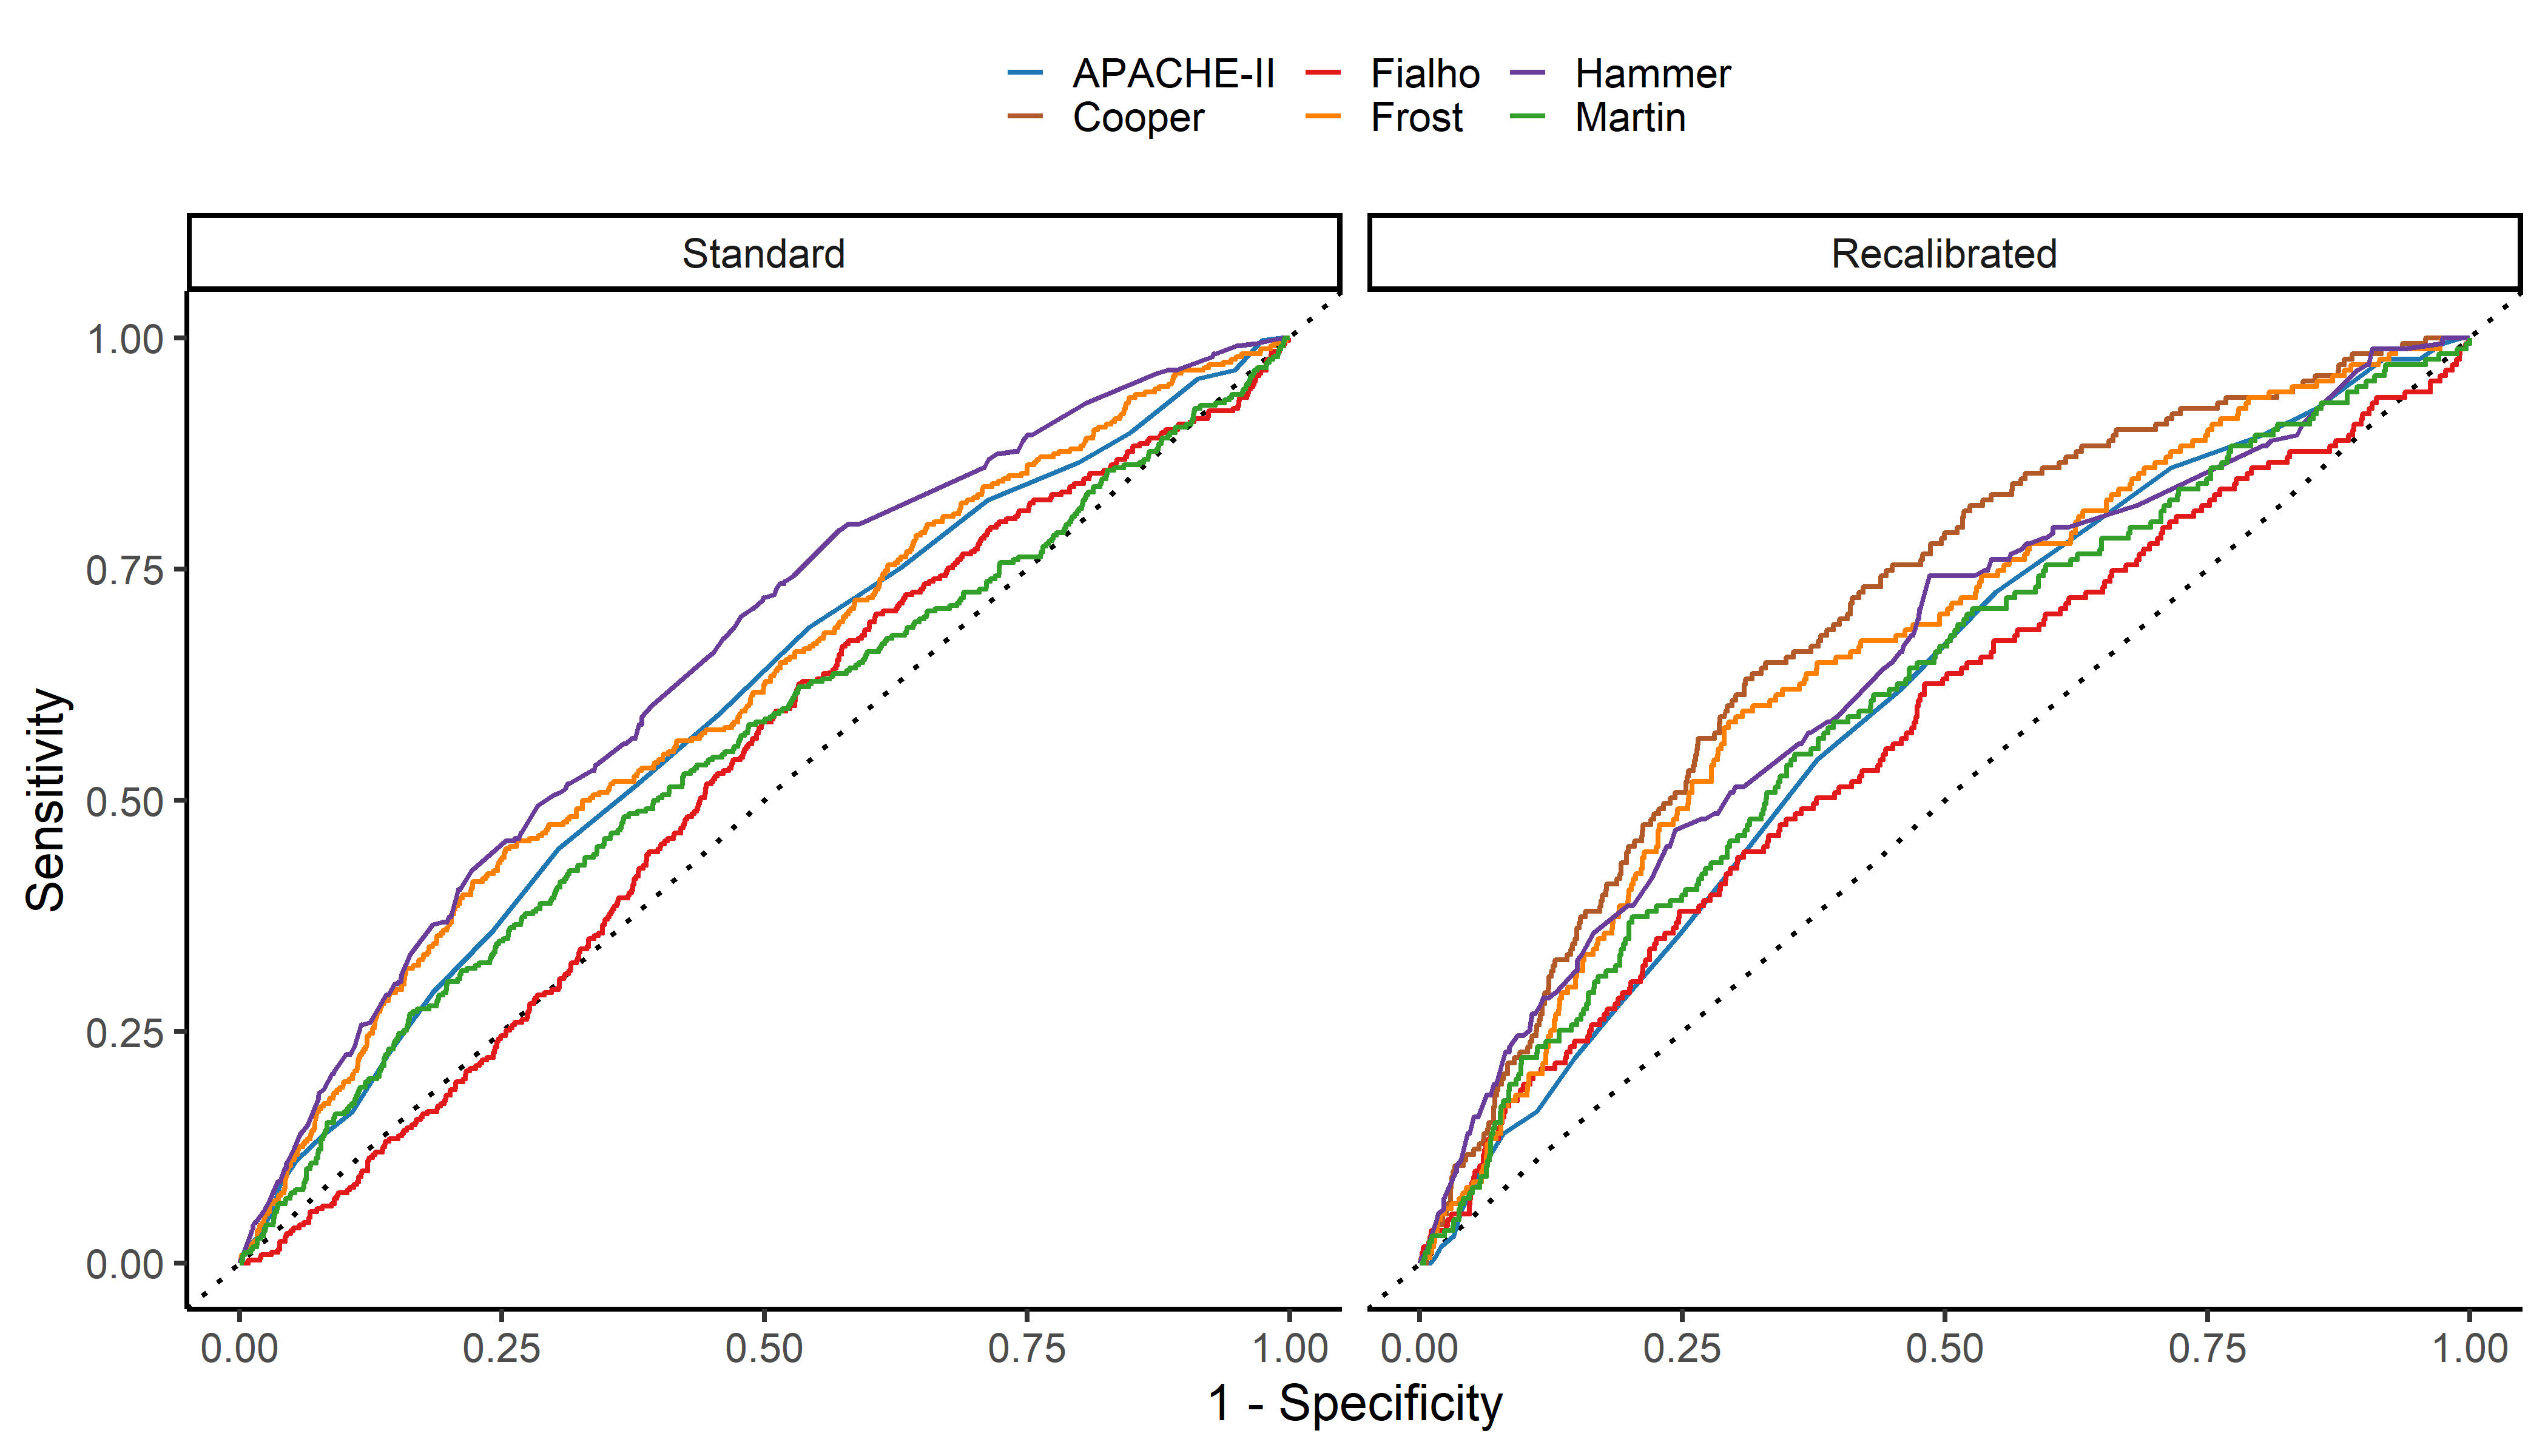
\includegraphics[width=\textwidth]{discrimination.png}
	\caption{}
	\label{DiscriminationFig}
\end{figure}


\subsection{Calibration}

% Overview of calibration, before and after recalibration
%	Above the line == under-prediction,  below == overprediction

% Calibration figure (standard and recalibrated
\begin{figure}
\centering
	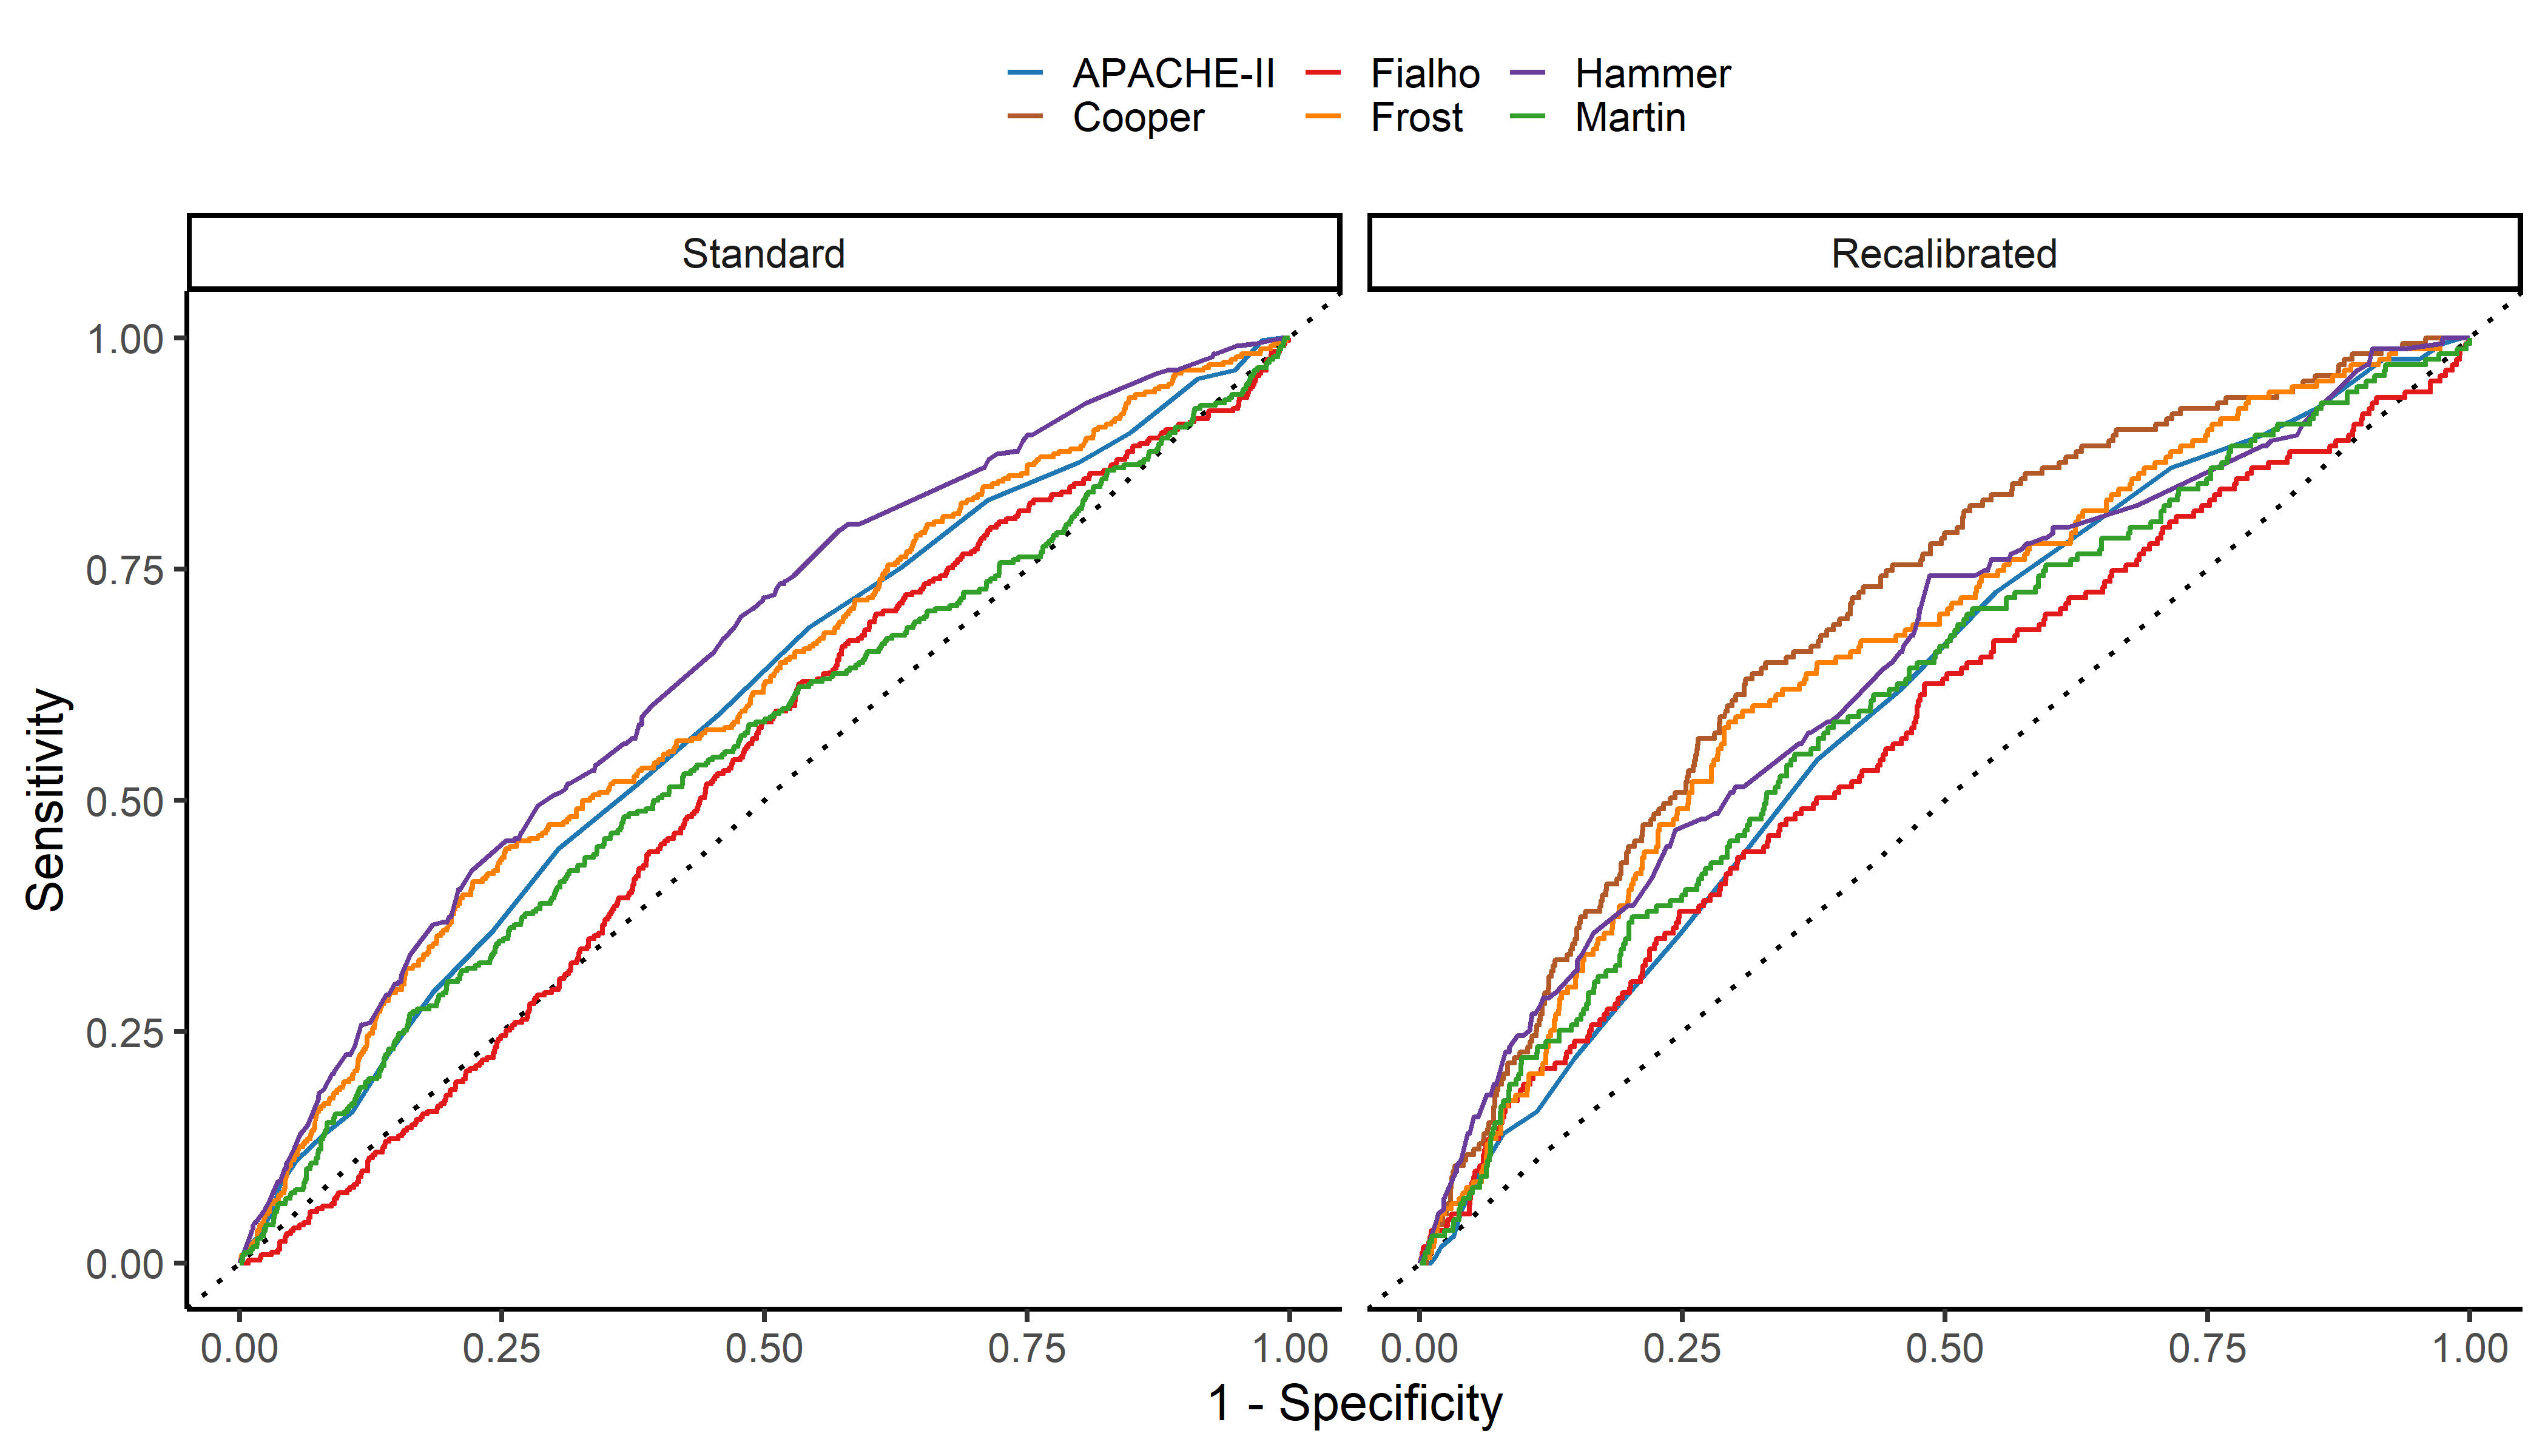
\includegraphics[width=\textwidth]{calibration.png}
	\caption{}
	\label{CalibrationFig}
\end{figure}

\subsection{Variables retained in novel model}

\section{Discussion}

\subsection{Model performance}

% Summarise above, make comparisons

\subsection{Next steps}

% Models to be taken forward

\begin{multicols}{2}
\bibliographystyle{thesis}
{\small
\bibliography{ICU_refs}}

\end{multicols}
\end{document}
